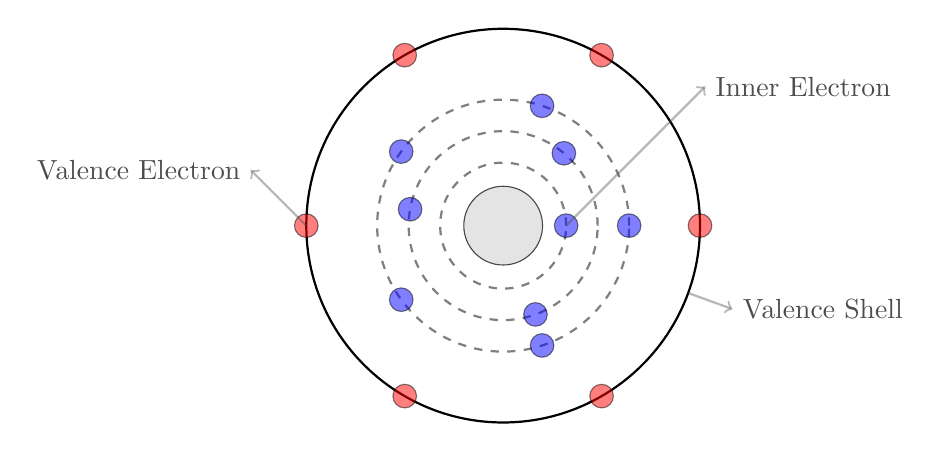
\begin{tikzpicture}[scale=1]

  % Atom nucleus
  \draw[fill=gray!30, opacity=0.7] (0,0) circle (0.5);
  
  % 1st orbit
  \draw[thick, dashed, opacity=0.5] (0,0) circle (0.8);
  \draw[fill=blue, opacity=0.5] (0:0.8) circle (0.15);
  
  % 2nd orbit
  \draw[thick, dashed, opacity=0.5] (0,0) circle (1.2);
  \foreach \angle in {50,170,290}
    \draw[fill=blue, opacity=0.5] (\angle:1.2) circle (0.15);
  
  % 3rd orbit
  \draw[thick, dashed, opacity=0.5] (0,0) circle (1.6);
  \foreach \angle in {72, 144, 216, 288, 360}
    \draw[fill=blue, opacity=0.5] (\angle:1.6) circle (0.15);
  
  % Valence shell (4th orbit)
  \draw[thick] (0,0) circle (2.5);
  \foreach \angle in {60, 120, 180, 240, 300, 360}
    \draw[fill=red, opacity=0.5] (\angle:2.5) circle (0.15);
  
  % Arrow pointing out one inner electron (longer)
  \draw[->, thick, black!70, opacity=0.4] (0:0.8) -- ++(45:2.5) node[right, text opacity=1] {Inner Electron};
  
  % Arrow pointing out one valence electron
  \draw[->, thick, black!70, opacity=0.4] (180:2.5) -- ++(135:1) node[left, text opacity=1] {Valence Electron};
  
  % Arrows describing the outermost orbit
  \draw[->, thick, black!70, opacity=0.4] (340:2.5) -- ++(340:0.6) node[right, text opacity=1] {Valence Shell};
  
  \end{tikzpicture}
  